\documentclass{standalone}
\usepackage{tikz}
\usetikzlibrary{patterns, positioning}

\begin{document}
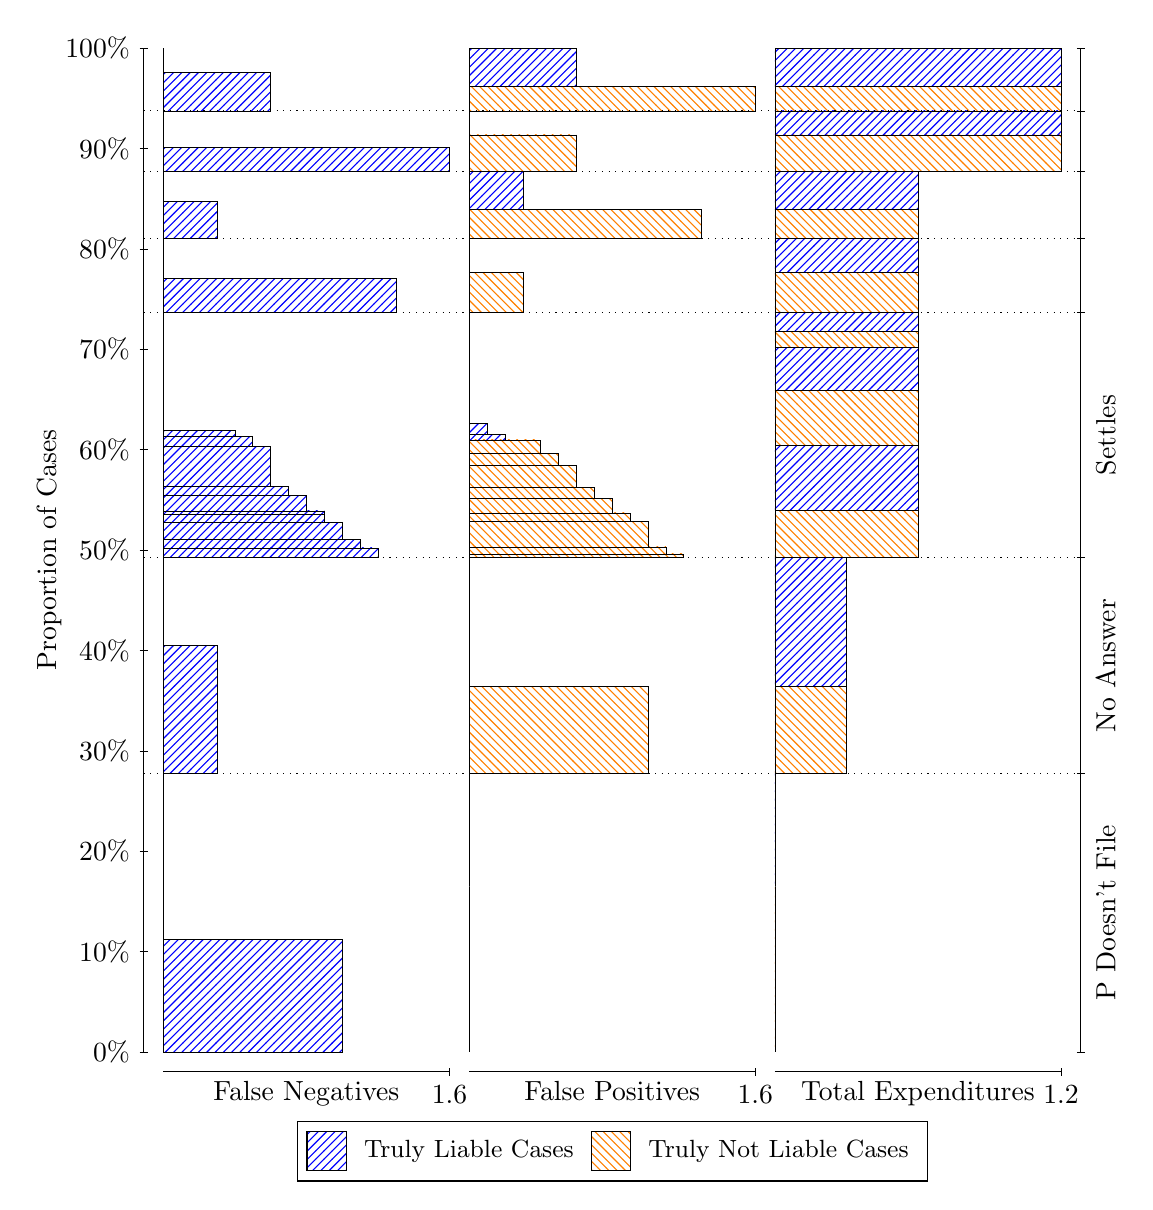
\begin{tikzpicture}
\draw[black, very thin] (1.5,1.75) -- (1.5,14.5);
\node[rotate=90, anchor=center] at (0.3, 8.125) {Proportion of Cases};
\draw[black, very thin] (1.45,1.75) -- (1.55,1.75);
\node[anchor=east] at (1.45, 1.75) {0\%};
\draw[black, very thin] (1.45,3.025) -- (1.55,3.025);
\node[anchor=east] at (1.45, 3.025) {10\%};
\draw[black, very thin] (1.45,4.3) -- (1.55,4.3);
\node[anchor=east] at (1.45, 4.3) {20\%};
\draw[black, very thin] (1.45,5.575) -- (1.55,5.575);
\node[anchor=east] at (1.45, 5.575) {30\%};
\draw[black, very thin] (1.45,6.85) -- (1.55,6.85);
\node[anchor=east] at (1.45, 6.85) {40\%};
\draw[black, very thin] (1.45,8.125) -- (1.55,8.125);
\node[anchor=east] at (1.45, 8.125) {50\%};
\draw[black, very thin] (1.45,9.4) -- (1.55,9.4);
\node[anchor=east] at (1.45, 9.4) {60\%};
\draw[black, very thin] (1.45,10.675) -- (1.55,10.675);
\node[anchor=east] at (1.45, 10.675) {70\%};
\draw[black, very thin] (1.45,11.95) -- (1.55,11.95);
\node[anchor=east] at (1.45, 11.95) {80\%};
\draw[black, very thin] (1.45,13.225) -- (1.55,13.225);
\node[anchor=east] at (1.45, 13.225) {90\%};
\draw[black, very thin] (1.45,14.5) -- (1.55,14.5);
\node[anchor=east] at (1.45, 14.5) {100\%};

\draw[black, very thin] (13.4,1.75) -- (13.4,14.5);
\draw[black, very thin] (13.35,1.75) -- (13.45,1.75);
\node[anchor=west] at (13.35, 1.75) {};
\draw[black, very thin] (13.35,5.2834) -- (13.45,5.2834);
\node[anchor=west] at (13.35, 5.2834) {};
\draw[black, very thin] (13.35,8.0283) -- (13.45,8.0283);
\node[anchor=west] at (13.35, 8.0283) {};
\draw[black, very thin] (13.35,11.14) -- (13.45,11.14);
\node[anchor=west] at (13.35, 11.14) {};
\draw[black, very thin] (13.35,12.081) -- (13.45,12.081);
\node[anchor=west] at (13.35, 12.081) {};
\draw[black, very thin] (13.35,12.929) -- (13.45,12.929);
\node[anchor=west] at (13.35, 12.929) {};
\draw[black, very thin] (13.35,13.702) -- (13.45,13.702);
\node[anchor=west] at (13.35, 13.702) {};
\draw[black, very thin] (13.35,14.5) -- (13.45,14.5);
\node[anchor=west] at (13.35, 14.5) {};

\draw[black, very thin, pattern color=blue, pattern=north east lines] (1.75,1.75) rectangle (4.0208,3.1837);
\draw[black, very thin, pattern color=orange, pattern=north west lines] (1.75,3.1837) rectangle (1.75,5.2834);
\draw[black, very thin, pattern color=blue, pattern=north east lines] (1.75,5.2834) rectangle (2.4312,6.9145);
\draw[black, very thin, pattern color=orange, pattern=north west lines] (1.75,6.9145) rectangle (1.75,8.0283);
\draw[black, very thin, pattern color=blue, pattern=north east lines] (1.75,8.0283) rectangle (4.475,8.1524);
\draw[black, very thin, pattern color=blue, pattern=north east lines] (1.75,8.1524) rectangle (4.2479,8.2616);
\draw[black, very thin, pattern color=blue, pattern=north east lines] (1.75,8.2616) rectangle (4.0208,8.4715);
\draw[black, very thin, pattern color=blue, pattern=north east lines] (1.75,8.4715) rectangle (3.7937,8.5756);
\draw[black, very thin, pattern color=blue, pattern=north east lines] (1.75,8.5756) rectangle (3.7937,8.6225);
\draw[black, very thin, pattern color=blue, pattern=north east lines] (1.75,8.6225) rectangle (3.5667,8.8196);
\draw[black, very thin, pattern color=blue, pattern=north east lines] (1.75,8.8196) rectangle (3.3396,8.9366);
\draw[black, very thin, pattern color=blue, pattern=north east lines] (1.75,8.9366) rectangle (3.1125,9.4396);
\draw[black, very thin, pattern color=blue, pattern=north east lines] (1.75,9.4396) rectangle (2.8854,9.5717);
\draw[black, very thin, pattern color=blue, pattern=north east lines] (1.75,9.5717) rectangle (2.6583,9.6449);
\draw[black, very thin, pattern color=orange, pattern=north west lines] (1.75,9.6449) rectangle (1.75,11.14);
\draw[black, very thin, pattern color=blue, pattern=north east lines] (1.75,11.14) rectangle (4.7021,11.57);
\draw[black, very thin, pattern color=orange, pattern=north west lines] (1.75,11.57) rectangle (1.75,12.081);
\draw[black, very thin, pattern color=blue, pattern=north east lines] (1.75,12.081) rectangle (2.4312,12.556);
\draw[black, very thin, pattern color=orange, pattern=north west lines] (1.75,12.556) rectangle (1.75,12.929);
\draw[black, very thin, pattern color=blue, pattern=north east lines] (1.75,12.929) rectangle (5.3833,13.235);
\draw[black, very thin, pattern color=orange, pattern=north west lines] (1.75,13.235) rectangle (1.75,13.702);
\draw[black, very thin, pattern color=blue, pattern=north east lines] (1.75,13.702) rectangle (3.1125,14.186);
\draw[black, very thin, pattern color=orange, pattern=north west lines] (1.75,14.186) rectangle (1.75,14.5);
\draw[black, very thin, pattern color=orange, pattern=north west lines] (5.6333,1.75) rectangle (5.6333,3.8497);
\draw[black, very thin, pattern color=blue, pattern=north east lines] (5.6333,3.8497) rectangle (5.6333,5.2834);
\draw[black, very thin, pattern color=orange, pattern=north west lines] (5.6333,5.2834) rectangle (7.9042,6.3972);
\draw[black, very thin, pattern color=blue, pattern=north east lines] (5.6333,6.3972) rectangle (5.6333,8.0283);
\draw[black, very thin, pattern color=orange, pattern=north west lines] (5.6333,8.0283) rectangle (8.3583,8.0757);
\draw[black, very thin, pattern color=orange, pattern=north west lines] (5.6333,8.0757) rectangle (8.1313,8.1635);
\draw[black, very thin, pattern color=orange, pattern=north west lines] (5.6333,8.1635) rectangle (7.9042,8.4909);
\draw[black, very thin, pattern color=orange, pattern=north west lines] (5.6333,8.4909) rectangle (7.6771,8.5972);
\draw[black, very thin, pattern color=orange, pattern=north west lines] (5.6333,8.5972) rectangle (7.45,8.7798);
\draw[black, very thin, pattern color=orange, pattern=north west lines] (5.6333,8.7798) rectangle (7.2229,8.9178);
\draw[black, very thin, pattern color=orange, pattern=north west lines] (5.6333,8.9178) rectangle (6.9958,9.203);
\draw[black, very thin, pattern color=orange, pattern=north west lines] (5.6333,9.203) rectangle (6.7687,9.3479);
\draw[black, very thin, pattern color=orange, pattern=north west lines] (5.6333,9.3479) rectangle (6.5417,9.5239);
\draw[black, very thin, pattern color=blue, pattern=north east lines] (5.6333,9.5239) rectangle (6.0875,9.597);
\draw[black, very thin, pattern color=blue, pattern=north east lines] (5.6333,9.597) rectangle (5.8604,9.7291);
\draw[black, very thin, pattern color=blue, pattern=north east lines] (5.6333,9.7291) rectangle (5.6333,11.14);
\draw[black, very thin, pattern color=orange, pattern=north west lines] (5.6333,11.14) rectangle (6.3146,11.652);
\draw[black, very thin, pattern color=blue, pattern=north east lines] (5.6333,11.652) rectangle (5.6333,12.081);
\draw[black, very thin, pattern color=orange, pattern=north west lines] (5.6333,12.081) rectangle (8.5854,12.454);
\draw[black, very thin, pattern color=blue, pattern=north east lines] (5.6333,12.454) rectangle (6.3146,12.929);
\draw[black, very thin, pattern color=orange, pattern=north west lines] (5.6333,12.929) rectangle (6.9958,13.396);
\draw[black, very thin, pattern color=blue, pattern=north east lines] (5.6333,13.396) rectangle (5.6333,13.702);
\draw[black, very thin, pattern color=orange, pattern=north west lines] (5.6333,13.702) rectangle (9.2667,14.016);
\draw[black, very thin, pattern color=blue, pattern=north east lines] (5.6333,14.016) rectangle (6.9958,14.5);
\draw[black, very thin, pattern color=orange, pattern=north west lines] (9.5167,1.75) rectangle (9.5167,3.8497);
\draw[black, very thin, pattern color=blue, pattern=north east lines] (9.5167,3.8497) rectangle (9.5167,5.2834);
\draw[black, very thin, pattern color=orange, pattern=north west lines] (9.5167,5.2834) rectangle (10.425,6.3972);
\draw[black, very thin, pattern color=blue, pattern=north east lines] (9.5167,6.3972) rectangle (10.425,8.0283);
\draw[black, very thin, pattern color=orange, pattern=north west lines] (9.5167,8.0283) rectangle (11.333,8.626);
\draw[black, very thin, pattern color=blue, pattern=north east lines] (9.5167,8.626) rectangle (11.333,9.4582);
\draw[black, very thin, pattern color=orange, pattern=north west lines] (9.5167,9.4582) rectangle (11.333,10.154);
\draw[black, very thin, pattern color=blue, pattern=north east lines] (9.5167,10.154) rectangle (11.333,10.702);
\draw[black, very thin, pattern color=orange, pattern=north west lines] (9.5167,10.702) rectangle (11.333,10.903);
\draw[black, very thin, pattern color=blue, pattern=north east lines] (9.5167,10.903) rectangle (11.333,11.14);
\draw[black, very thin, pattern color=orange, pattern=north west lines] (9.5167,11.14) rectangle (11.333,11.652);
\draw[black, very thin, pattern color=blue, pattern=north east lines] (9.5167,11.652) rectangle (11.333,12.081);
\draw[black, very thin, pattern color=orange, pattern=north west lines] (9.5167,12.081) rectangle (11.333,12.454);
\draw[black, very thin, pattern color=blue, pattern=north east lines] (9.5167,12.454) rectangle (11.333,12.929);
\draw[black, very thin, pattern color=orange, pattern=north west lines] (9.5167,12.929) rectangle (13.15,13.396);
\draw[black, very thin, pattern color=blue, pattern=north east lines] (9.5167,13.396) rectangle (13.15,13.702);
\draw[black, very thin, pattern color=orange, pattern=north west lines] (9.5167,13.702) rectangle (13.15,14.016);
\draw[black, very thin, pattern color=blue, pattern=north east lines] (9.5167,14.016) rectangle (13.15,14.5);
\draw[black, dotted] (1.5,5.2834) -- (13.4,5.2834);
\draw[black, dotted] (1.5,8.0283) -- (13.4,8.0283);
\draw[black, dotted] (1.5,11.14) -- (13.4,11.14);
\draw[black, dotted] (1.5,12.081) -- (13.4,12.081);
\draw[black, dotted] (1.5,12.929) -- (13.4,12.929);
\draw[black, dotted] (1.5,13.702) -- (13.4,13.702);
\draw[black, very thin] (1.75,1.5) -- (5.3833,1.5);
\node[anchor=north] at (3.5667, 1.5) {False Negatives};
\draw[black, very thin] (5.3833,1.45) -- (5.3833,1.55);
\node[anchor=north] at (5.3833, 1.45) {1.6};

\draw[black, very thin] (5.6333,1.5) -- (9.2667,1.5);
\node[anchor=north] at (7.45, 1.5) {False Positives};
\draw[black, very thin] (9.2667,1.45) -- (9.2667,1.55);
\node[anchor=north] at (9.2667, 1.45) {1.6};

\draw[black, very thin] (9.5167,1.5) -- (13.15,1.5);
\node[anchor=north] at (11.333, 1.5) {Total Expenditures};
\draw[black, very thin] (13.15,1.45) -- (13.15,1.55);
\node[anchor=north] at (13.15, 1.45) {1.2};

\node[black, centered, rotate=90] at (13.72, 3.5167) {P Doesn't File};
\node[black, centered, rotate=90] at (13.72, 6.6558) {No Answer};
\node[black, centered, rotate=90] at (13.72, 9.5844) {Settles};





\draw (7.449999999999999,1.5) node[draw=none] (baseCoordinate) {};
\begin{scope}[align=center]
        \matrix[scale=0.5, draw=black, below=0.5cm of baseCoordinate, nodes={draw}, column sep=0.1cm]{
            \node[rectangle, draw, minimum width=0.5cm, minimum height=0.5cm, pattern=north east lines, pattern color=blue] {}; &
            \node[draw=none, font=\small] (B) {Truly Liable Cases}; &
            \node[rectangle, draw, minimum width=0.5cm, minimum height=0.5cm, pattern=north west lines, pattern color=orange] {}; &
            \node[draw=none, font=\small] (B) {Truly Not Liable Cases}; \\
            };
\end{scope}

\end{tikzpicture}
\end{document}